\documentclass[journal]{vgtc}                % final (journal style)
%\documentclass[review,journal]{vgtc}         % review (journal style)
%\documentclass[widereview]{vgtc}             % wide-spaced review
%\documentclass[preprint,journal]{vgtc}       % preprint (journal style)

%% Uncomment one of the lines above depending on where your paper is
%% in the conference process. ``review'' and ``widereview'' are for review
%% submission, ``preprint'' is for pre-publication, and the final version
%% doesn't use a specific qualifier.

%% Please use one of the ``review'' options in combination with the
%% assigned online id (see below) ONLY if your paper uses a double blind
%% review process. Some conferences, like IEEE Vis and InfoVis, have NOT
%% in the past.

%% Please use the ``preprint''  option when producing a preprint version
%% for sharing your article on an open access repository

%% Please note that the use of figures other than the optional teaser is not permitted on the first page
%% of the journal version.  Figures should begin on the second page and be
%% in CMYK or Grey scale format, otherwise, colour shifting may occur
%% during the printing process.  Papers submitted with figures other than the optional teaser on the
%% first page will be refused. Also, the teaser figure should only have the
%% width of the abstract as the template enforces it.

%% These few lines make a distinction between latex and pdflatex calls and they
%% bring in essential packages for graphics and font handling.
%% Note that due to the \DeclareGraphicsExtensions{} call it is no longer necessary
%% to provide the the path and extension of a graphics file:
%% \includegraphics{diamondrule} is completely sufficient.
%%
\ifpdf%                                % if we use pdflatex
  \pdfoutput=1\relax                   % create PDFs from pdfLaTeX
  \pdfcompresslevel=9                  % PDF Compression
  \pdfoptionpdfminorversion=7          % create PDF 1.7
  \ExecuteOptions{pdftex}
  \usepackage{graphicx}                % allow us to embed graphics files
  \DeclareGraphicsExtensions{.pdf,.png,.jpg,.jpeg} % for pdflatex we expect .pdf, .png, or .jpg files
\else%                                 % else we use pure latex
  \ExecuteOptions{dvips}
  \usepackage{graphicx}                % allow us to embed graphics files
  \DeclareGraphicsExtensions{.eps}     % for pure latex we expect eps files
\fi%

%% it is recomended to use ``\autoref{sec:bla}'' instead of ``Fig.~\ref{sec:bla}''
\graphicspath{{figures/}{pictures/}{images/}{./}} % where to search for the images

\usepackage{microtype}                 % use micro-typography (slightly more compact, better to read)
\PassOptionsToPackage{warn}{textcomp}  % to address font issues with \textrightarrow
\usepackage{textcomp}                  % use better special symbols
\usepackage{mathptmx}                  % use matching math font
\usepackage{times}                     % we use Times as the main font
\renewcommand*\ttdefault{txtt}         % a nicer typewriter font
\usepackage{cite}                      % needed to automatically sort the references
\usepackage{tabu}                      % only used for the table example
\usepackage{booktabs}                  % only used for the table example
%% We encourage the use of mathptmx for consistent usage of times font
%% throughout the proceedings. However, if you encounter conflicts
%% with other math-related packages, you may want to disable it.

%% In preprint mode you may define your own headline. If not, the default IEEE copyright message will appear in preprint mode.
%\preprinttext{To appear in IEEE Transactions on Visualization and Computer Graphics.}

%% In preprint mode, this adds a link to the version of the paper on IEEEXplore
%% Uncomment this line when you produce a preprint version of the article 
%% after the article receives a DOI for the paper from IEEE
%\ieeedoi{xx.xxxx/TVCG.201x.xxxxxxx}

%% If you are submitting a paper to a conference for review with a double
%% blind reviewing process, please replace the value ``0'' below with your
%% OnlineID. Otherwise, you may safely leave it at ``0''.
\onlineid{0}

%% declare the category of your paper, only shown in review mode
\vgtccategory{Research}
%% please declare the paper type of your paper to help reviewers, only shown in review mode
%% choices:
%% * algorithm/technique
%% * application/design study
%% * evaluation
%% * system
%% * theory/model
\vgtcpapertype{application/design study}

\title{Augmented Reality Relating to GPS Navigation for Pilot Navigation and Orientation}


\author{
  Daniel de Paz}
\authorfooter{
%% insert punctuation at end of each item
\item
 Daniel de Paz is an undergraduate student at Colorado State University.
}
%TODO do I need this??????????????

%other entries to be set up for journal
%\shortauthortitle{Biv \MakeLowercase{\textit{et al.}}: Global Illumination for Fun and Profit}
%\shortauthortitle{Firstauthor \MakeLowercase{\textit{et al.}}: Paper Title}

%% Abstract section.
%\abstract{
 %NO NEED 
%} % end of abstract

%% Keywords that describe your work. Will show as 'Index Terms' in journal
%% please capitalize first letter and insert punctuation after last keyword
%\keywords{Radiosity, global illumination, constant time}
%NO NEED

%\CCScatlist{ % not used in journal version
% \CCScat{K.6.1}{Management of Computing and Information Systems}%
%{Project and People Management}{Life Cycle};
% \CCScat{K.7.m}{The Computing Profession}{Miscellaneous}{Ethics}
%}

%% A teaser figure can be included as follows
\teaser{
  \centering
  \includegraphics[width=\linewidth]{Denver}
  \caption{Flying Over Denver}
  \label{fig:teaser}
}

%% Uncomment below to disable the manuscript note
\renewcommand{\manuscriptnotetxt}{}

%% Copyright space is enabled by default as required by guidelines.
%% It is disabled by the 'review' option or via the following command:
 \nocopyrightspace


\vgtcinsertpkg

%%%%%%%%%%%%%%%%%%%%%%%%%%%%%%%%%%%%%%%%%%%%%%%%%%%%%%%%%%%%%%%%
%%%%%%%%%%%%%%%%%%%%%% START OF THE PAPER %%%%%%%%%%%%%%%%%%%%%%
%%%%%%%%%%%%%%%%%%%%%%%%%%%%%%%%%%%%%%%%%%%%%%%%%%%%%%%%%%%%%%%%%

\begin{document}

\firstsection{Introduction}

\maketitle

Aviation is one of the most important modes of transportation in the modern era. Whether through comercial liners or recreational puddle jumpers, aviation has become a staple of transportation. Nonetheless, there is a set amount of risk involved when flying. Mechanical failure, weather, animals, and midair collisions are an inherent factor that comes with flying. Most safety systems today can help limit these risks. Modern safety procedures do an excellent job from the ground to ensure safety but from the air, safety measures can be improved upon. The goal of this project is to not only to provide a way of identifying airports using Augmented Reality via a Heads Up Display (HUD), but to do so using resources within the airplane itself and not from other sources. HUDs in the aviation industry are used in modern fighter planes to identify enemy aircraft \cite{964244}. The goal of this project is to build a prototype HUD display for airports for small commercial and recreational planes.

\section{Current Instrumentations}

There are many different ways to land an airplane. When pilots are unable to land the plane visually, they can turn to multiple methods. The main landing assistant methods out there today are Instrument Landing System (ILS), GPS, Ground Based Augmentation Systems (GBAS), and Satellite Based Augmentation Systems (SBAS). While all of these systems work well in their own right, none of them are based within the aircraft itself. ILS is an analog way of lining up with the actual runway, not identifying where the runway is. This method has been widely used since it became standard in 1949. It uses lights at specified angles to direct the incoming landing path with proper decent angles and centering. If the incoming plane is at too low of an altitude, some of the lights will not be visible. If the altitude is too high, noo many of the lights are visible. The same is with centering with the runway. If too far to the left, the right lights become no longer visible \cite{8769357, 4586415, 8973154, 4068739}. While an effective system, its main purpose is to land the planes on the runway and not identify and guide the plane to the airport itself. 

GPS can identify the location of the airport and direction of the runway but current systems don’t utilize the actual surroundings in the instrument. GBAS uses GPS and a VHF radio to communicate with the aircraft and identify to growns crew the position of the aircraft \cite{murfin_2011, 4106292, 4745647, 4745660}. This requires the aircraft to be equipped with a VHF receiver. 

SBAS is still in its development stage. It is not reliable enough to be used on a large scale. Issues such as positioning errors, weather effects, and radio interference has kept this system from being implemented globally\cite{6184264}.

While GPS can be useful, GPS just uses the basic map scheme without any real world features like landmarks. When flying in a dense area like a mountain range, GBAS, SBAS, and GPS can have interference due to the geological challenges in the area.

\section{Project Plan}

The project will be done using the AR abilities of Unity through a phone. I have no experience coding Augmented Reality but I have experience with unity so it will be a useful base to learn. Phones have multiple useful instruments that can be useful to find position, direction, and display targets. Since this is a solo project, having some stable footing to start from is essential. The project will be broken up into two parts.

	The first and most important part of this project is getting a good understanding of augmented reality within Unity. So getting a basic program to display an object through the phone is the first step. Being able to display an object at a specific position while having a varying elevation and distance factor will take some time to figure out. 
	The second part will be to find a way to pull data of locations of airports and ourselves. Once the data can be pulled, it will be added to the object for positioning. Like pinning a location on an interactive map, the HUD of the phone will have the object pop up at those locations. 


\section{Utilized Technology}

The majority of technology utilized will be through the phone. The goal is to use augmented reality to create the waypoints. The phone will act as a Heads Up Display for the project. The phone’s GPS will be used for gathering data for both location and elevation. The elevation and positioning will be needed to coordinate pin locations for the airport popups. The camera and gyroscope of the phone will also be utilized for the augmented reality to direct the location and direction of the airports and overlay it with the surroundings.

\section{Methodology}

The Augmented Reality interactable objects were created using Unity for use on an android. Androids have a built in camera and gps needed for location and AR mapping. The goal was to create a popup for the user to identify locations when flying a plane without having to visually identify them. The idea is that if there were an emergency, the pilots could use this to identify where a runway is without any visibility or other instruments.

Subjects would be given 30 seconds to identify a location visually and another similar location within the general area via the prototype. This was repeated 5 different times with the same participant. 

After the flight, the participants answered a survey. The survey questions were as follows:

\begin{itemize}
  \item On a scale of 1 to 10, rate the usability of the prototype
  \item Note any comments about the usability of the prototype
  \item On a scale of 1 to 10, rate the usefulness of the prototype
  \item Note any comments about the usefulness of the prototype
  \item On a scale of 1 to 10, rate the identifiability of the location objects within the prototype
  \item Note any comments about the identifiability of the location objects within the prototype
  \item On a scale of 1 to 10, how likely would you use this prototype if it were released?
  \item How does the prototype compare to visual identification methods?
  \item Note any final opinions, suggestions, or preferable changes to the system
\end{itemize}


For this particular experiment, the plan is to use 5 subjects due to limitations in finding able bodied people to fly with. This low number is due to the researcher’s limited network of willing known pilots. This small testing pool is not advised if this experiment is reproduced as a low amount of subjects can cause distorted results.

For these flights, we used small, single prop planes to fly in as seen in Figure ~\ref{fig:josh}.

\begin{figure}[tb]
  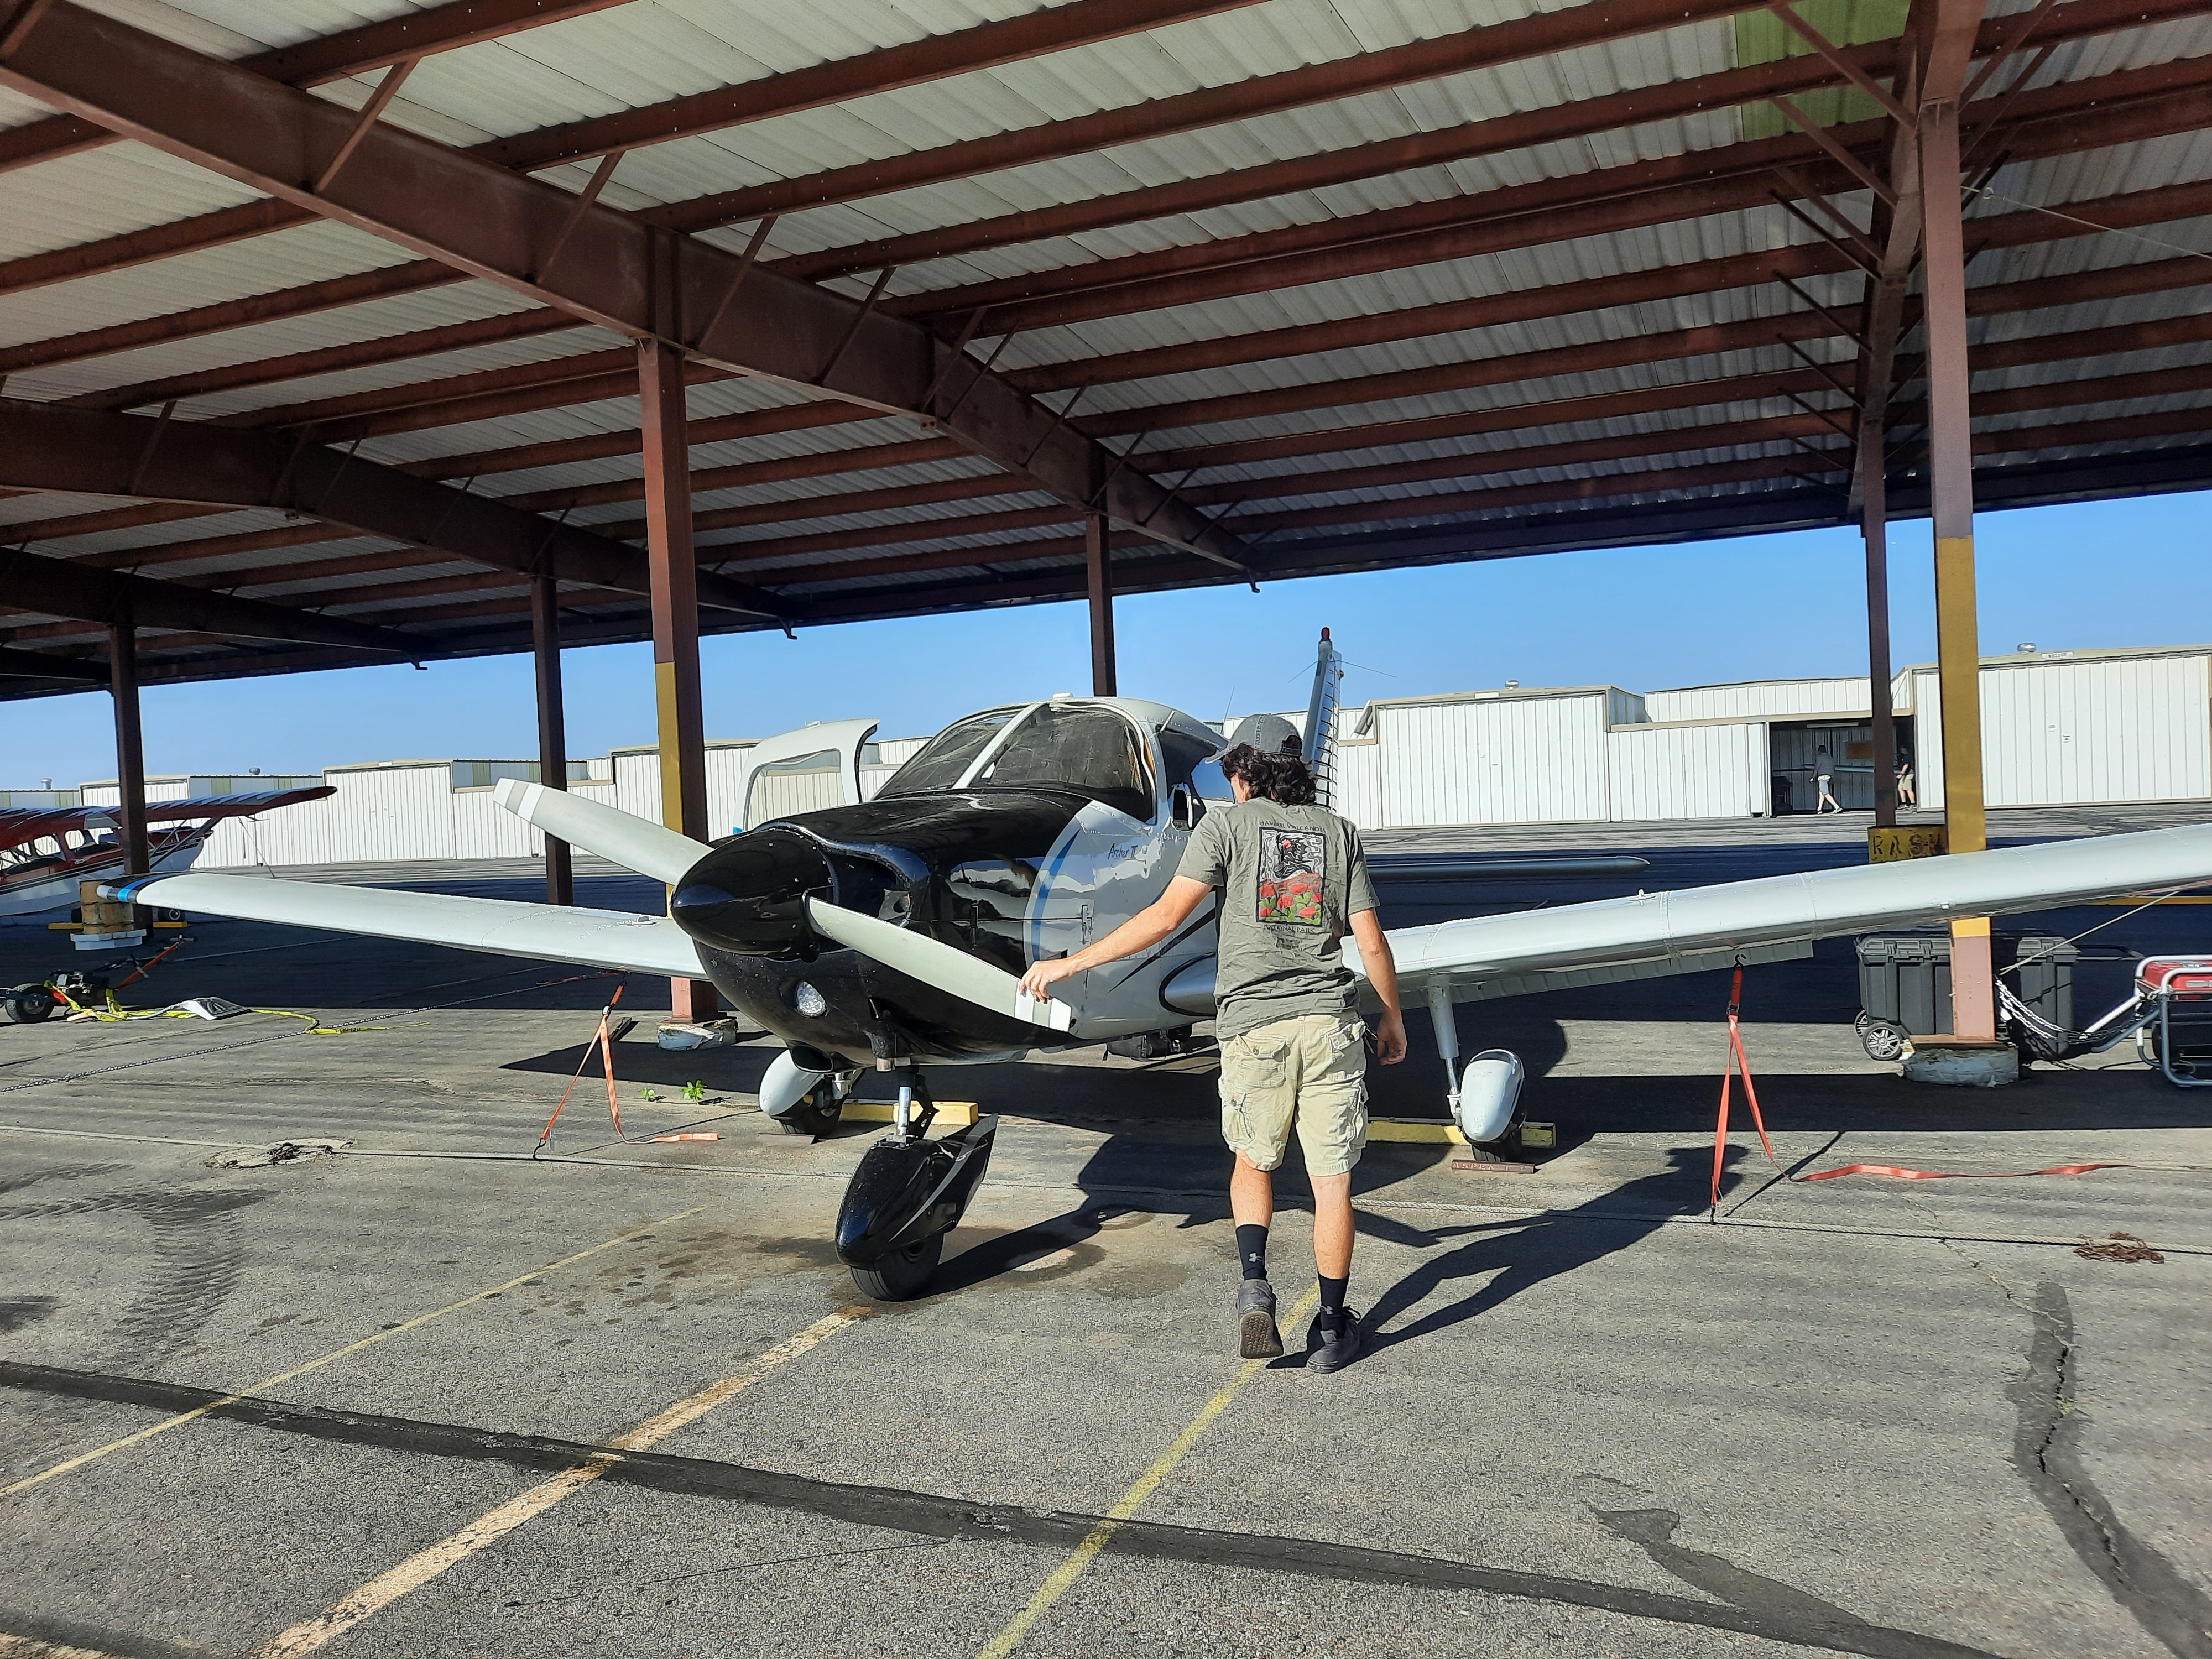
\includegraphics[width=\columnwidth]{Josh.jpg}
  \caption{Pilot doing preflight checks on the plane}
  \label{fig:josh}
\end{figure}

\begin{figure}[tb]
  \includegraphics[width=\columnwidth]{CSU.jpg}
  \caption{Example implimentation with Colorado State as the target}
  \label{fig:csu}
\end{figure}

\section{Analysis}
Due to weather conflicts, we were unable to fly the last scheduled flight before the deadline. Because of this, there were only 3 tested participants. 

\begin{table}
  \caption{Servey of Prototype Testing}
  \label{tab:servey}
  \scriptsize%
	\centering%
  \begin{tabu}{%
	r%
	*{4}{c}%
	*{2}{r}%
	}
  \toprule
   participant & \rotatebox{90}{Usability} &   \rotatebox{90}{usefullness} &   \rotatebox{90}{Identifiability} &   \rotatebox{90}{Likelihood of being used}\\
  \midrule
	1 & 3 & 4 & 3 & 1 \\
  2 & 4 & 6 & 6 & 2 \\
  3 & 6 & 5 & 5 & 3 \\
  \midrule
  \textbf{avg} & \textbf{4.3} & \textbf{5} & \textbf{5.7} & \textbf{2} \\
  \bottomrule
  \end{tabu}%
\end{table}

The subjects rated the usability at a 4.3 with a max of a 6 and a min of 3. Notable marks were that there wasn’t a UI for actually using the product but once in the air, it was easy to look around within the plane and pan the system. Usefulness was rated a 5 out of 10. Main highlights noted were the ability to see markers even if they were in blindspots within the aircraft. Notable setbacks were the fact that this system is not handsfree in its current implementation.. Identifiability was rated a 5.7 out of 10. The likelihood of this prototype being used if released as is was rated 2 out of 10. Notes for the low score were due to the necessary improvements needed prior to an official release.

Notable comments for improvement of the system were as follows:
\begin{itemize}
  \item The gps was inconsistent
  \item Improved usability
  \item A wanting for a hands free option
  \item Colors blend in with landscape
  \item An improved identifying feature for the popups
\end{itemize}

\section{Limitations and Challenges}
There were a plethora of pitfalls and setbacks in development and testing of this prototype. Logistically, there was major difficulty getting into the air to run the test on the pilots. Unforeseen setbacks such as weather cancellations created issues in being able to run the experiment. When in the air, factors such as visibility and air quality as well as cloud coverage and daylight also played major roles in the outcome of this experiment. These unforeseen factors drastically affected the experiment and results in ways unanticipated. 

\section{Future Development}
In its current state, indications point to this not being a useful prototype. Improvements must be made in order to improve the usefulness of this product.

The original goal of this prototype is to identify airports for pilots in case of an emergency landing. Future developments would be to connect these location objects to a database of airports for a wider general use. This could be done by having the pilot set a route prior to takeoff so the application could pull from a database and plot nearby locations along the route. 

Further development to accommodate these comments would be necessary before any real world application could be viable. In order to make the program more user friendly, a whole UI system would need to be implemented. Different color schemes could be used to contrast the landscape. Making the popups selectable before the flight could make a primary target for the system to point towards. Making the popups blink slowly could help with identifying the selected destination. Eventually this system could be used as an integrated HUD on the glass enabling hands free viewing. Having the system integrated could then use the aircraft’s own instruments for guidance.


\section{Conclusion}

Aviation has a number of useful navigational tools. Most of these tools are ground based and not within the aircraft. By using augmented reality, this project is designed to give more control to the aircraft when it comes to navigation. Whether it is used for general navigation in complicated terrain like mountain ranges or quick navigation in case of an emergency, the goal of this project is to make navigation easier from the pilot’s perspective within the airplane.
%filler for now

%% if specified like this the section will be committed in review mode
%\acknowledgments{
%The authors wish to thank A, B, and C. This work was supported in part by
%a grant from XYZ (\# 12345-67890).}
%not needed

%\bibliographystyle{abbrv}
\bibliographystyle{abbrv-doi}
%\bibliographystyle{abbrv-doi-narrow}
%\bibliographystyle{abbrv-doi-hyperref}
%\bibliographystyle{abbrv-doi-hyperref-narrow}

\bibliography{template}
\end{document}

